\chapter{Motivation and Background}
\label{ch:motivation}

\section{Overview}
This chapter first...

\section{Energy Efficient Base Stations}
\label{sect:eebs}
A sample figure.

\begin{figure}
\centering
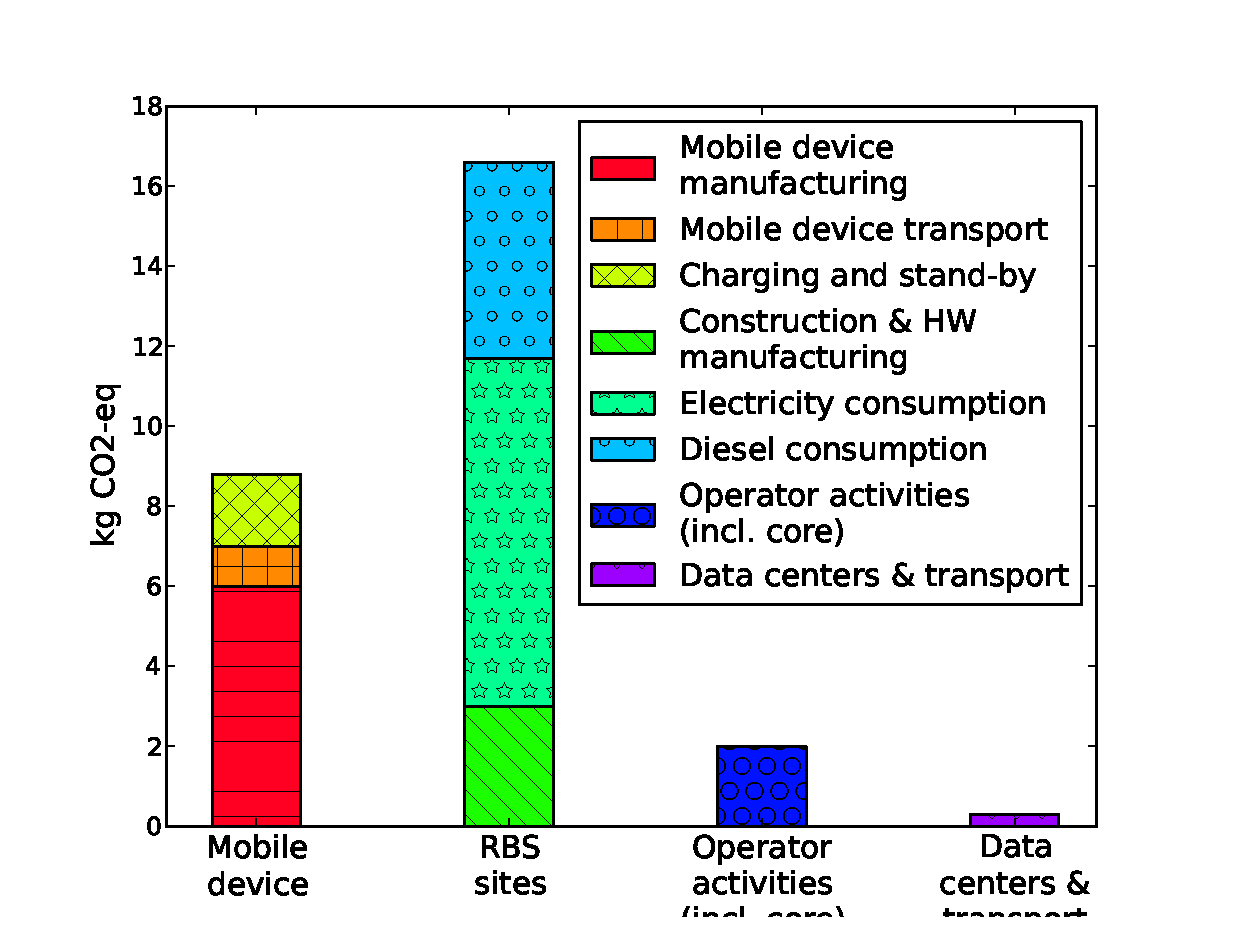
\includegraphics[width=0.6\textwidth]{\dir/img/carbonfootprint}
\caption[The carbon footprint for an average subscriber in 2007]{The carbon footprint (\coo-equivalent emissions, see Section~\ref{sect:quantEE}) for an average subscriber in 2007~\cite{mmlfl1001}.} % from enablers paper, my own. How to reference?
\label{fig:4}
\end{figure}

\section{Quantifying Energy Efficiency}
\label{sect:quantEE}
Enhancing the energy efficiency of communication networks has led to a field of research popularly labelled \emph{Green Radio}...

\section{Green Radio in Literature}
Historically, ...

\section{Technical Background}
\label{background}

The following sections outline some fundamental concepts ...

\subsection{\ac{LTE}}

\ac{LTE}~\cite{book:dps1101} is a wireless access standard superseding the \ac{GSM} and \ac{UMTS} for increased network capacities. 

\subsection{Multi-carrier Technology}
\label{sect:multicarrier}
The wireless medium is inherently shared...

\subsection{Network Simulation}

For many problems in communications research...

\section{Summary}
This chapter served to provide ...

